\lhead{\emph{Related work}}
\chapter{Related work}
In this chapter specific research areas and systems related to this thesis are presented. First the current situation on mobile music player user interfaces is discussed. Then a wider description of two research areas; mobile HCI and multimodal interaction are presented before going into details about how previous developed interaction techniques within these two areas can be combined with a mobile music player UI. A graphical overview is shown in fig. \ref{fig:venn}.

\begin{figure}[htbp]
	\centering
		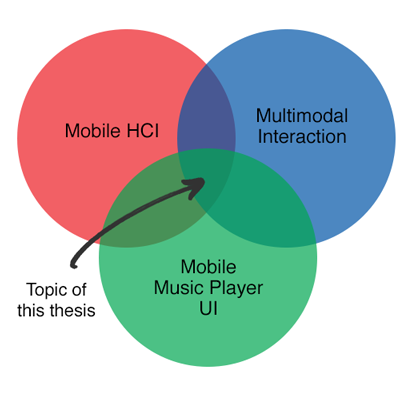
\includegraphics[width=0.5\textwidth,height=\textheight,keepaspectratio]{./Figures/venn.png}
		\rule{35em}{0.5pt}
	\caption[Venn diagram]{Thesis topic position}
	\label{fig:venn}
\end{figure}


\section{Mobile Music Player UI}
% Intro
Although mobile audio players have developed since the first portable cassette player by Sony in 1979 towards todays digital audio players with storage capacity e.g. smartphones, there is still one property that remains - the way in which we interact with the device. E.g. like we needed the hands and eyes for rewinding or turning the tape on a cassette player, we need them as well for swiping to the preferred track in our smartphone music application.

% Problems
Maybe some statistic about music listening on the go
Ref to chapter 1 when talking about distractions
Maybe add this: In these situations a vital factor is to minimize the amount of distraction for interaction modes \cite{pascoe_using_2000}

% Alternatives in music players
- iPod shuffle, no visual interface (not user decision)
- xpod, based on emotions... (not user decision)
- leg shifting music track while running \cite{smus_running_2010}
- body pose


\section{Mobile Human Computer Interaction}
[TODO]

\subsection{Interaction in motion}

- Cognitive load

\subsection{Mobil device limitations}


\section{Multimodal interaction}
[TODO: multimodal interaction in general]

- What kind of modalities, combinations

%\subsection{Hands-free interaction}
%This term refers to controlling a system without using the hands including no hand gestures. Achieving this hands-freeness interaction often relates to speech recognition or gaze/head tracking techniques but also other body parts are used for simple interactions e.g. leg shifting music track while running \cite{smus_running_2010}. Speech recognition is becoming a more common interaction modality but there exists accuracy and stability challenges especially in mobile noisy environments. In contrast head tracking could possibly provide a more stable interaction detection in mobile environments. [TODO: Last sentence rephrase and explain why you think this is the case]

\subsection{Eyes-free interaction}
Several work on both audio \cite{kajastila_eyes-free_2013,bonner_no-look_2010,brewster_multimodaleyes-freeinteraction_2003,zhao_earpod:_2007,vazquez-alvarez_eyes-free_2011} and haptic \cite{pasquero_haptic_2011,pielot_tactile_2011} displays use the term eyes-free which refers to controlling the state of a system without visual attention. This kind of interaction has shown to be desirable in some situations \cite{oakley_designing_2007,yi_exploring_2012} and even improve efficiency compaired to traditional visual displays \cite{zhao_earpod:_2007}.

% visual competition, concentration
One of the main motivations behind this eyes-free use is to design interfaces that do not compete with the users visual attention. That is this "visual competition" could introduce risks when people are on the move e.g. travelling in traffic. In these situations a vital factor is to minimize the amount of distraction for interaction modes \cite{pascoe_using_2000}. Eyes-free interfaces can keep the users visual attention on the road while driving \cite{sodnik_user_2008} or walking around in the city \cite{vazquez-alvarez_eyes-free_2011}. [TODO: rephrase, at this point you should also tell the reader about the complexity of human attention which can to some degree sometimes be decoupled from modalities and that just because information comes in a modality different from the one currently in use doesnt mean that it doesnt distract cognitively]

% visual display problems
Much of the interfaces work in wearable computing tends to focus on visual headmounted displays \cite{barfield_fundamentals_2000} e.g. Google Project Glass. But not only as mentioned does visual displays occupy the users visual attention, they can also be obtrusive and hard to use in bright daylight \cite{geelhoed_safety_2000}. Another disadvantage with visual displays is that their power consumption is high i.e. they drain a mobile device battery and they are expensive. By using eyes-free interfaces it is possible to use cheaper and less power consuming hardware.


\section{Spatial sound}
[TODO]

% motivation for audio and spatial sound feedback
William W. Gaver, a pioneer in audio interfaces, has explored several aspects of using sound in interfaces including the intuitiveness of presenting complex information to users in the form of audio \cite{gaver_sonicfinder:_1989}. Similarly Graham explores the advantages in reaction time when using ”auditory icons” \cite{graham_use_1999}. In \cite{gaver_auditory_1986} Gaver presents the use of spatial sound icons. In doing so, he draws forward the unutilized potential of creating natural interaction through spatial audio.

By compairing visual and audio feedback when pushing buttons on the same GUI, Brewster showed that it was difficult for users to devote all their visual attention to an interface while walking, running og driving and that the interaction workload decreased with audio feedback \cite{brewster_overcoming_2002}.

\subsection{Non-speech audio}
Work has shown that non-speech audio is effective in improving the interaction with mobile devices \cite{pirhonen_gestural_2002, sawhney_nomadic_2000}.

\subsection{Head Related Transfer Function}
[TODO]

Good reference for 3d sound \cite{begault_3dd_1994}


\section{Head gesture interaction}
There exists different kinds of approaches when it comes to controlling a system with head gestures. Using cameras it is possible to effectively track head movements via facial recognition \cite{morimoto_recognition_1996} and gaze tracking makes it possible to control an object by fixating the eyes on that object while moving the head \cite{mardanbegi_eye-based_2012}. Thus these techniques do not require any hardware sensors e.g. accelerometer and gyroscope but in return a camera placed in front of the user. [TODO: you need to explain this better. our recently graduated phd student diakonhas developed a wearable solution]

\subsection{Intelligent Headset}
[TODO]


\section{Related systems}
[TODO: intro]

% closely related to my project
Brewster et al. showed that novel interaction techniques based on sound and gesture can significantly improve the usability of a wearable device in particular under "eyes-free" mobile conditions and that head gestures was a successful interaction technique with egocentric sounds the most effective \cite{brewster_multimodaleyes-freeinteraction_2003}.

Park et al. also experimented, using head gesture input and aural output, with 1D and 2D menu interfaces \cite{park_gaze-directed_2011}.

Kajastila and Lokki has done a user study comparing auditory and visual menus controlled by the same free-hand gestures where the majority of the participants felt that an auditory circular menu was faster than a visual based menu \cite{kajastila_interaction_2013}.

\subsection{Systems properties overview}
[TODO]

Table compairing properties of related work (and this project) example fig. \ref{tab:related} (NOTE: temp, i need some input for this...).

\begin{table}[h] 
\caption{Related works properties comparison} % title name of the table 
%\centering % centering table

\begin{tabular}{L{4cm}C{2cm}C{2cm}C{2cm}C{2cm}} \toprule
    Related work & Head gesture interaction & Spatial sound feedback & Music application & Accessible hardware \\ \midrule
    Multimodal eyes-free interaction techniques for wearable devices \cite{brewster_multimodaleyes-freeinteraction_2003}  & + & + & - & - \\ \midrule
    This project  & + & + & + & + \\ \bottomrule
\end{tabular}

\label{tab:related} 
\end{table}










